\section{Specifying TGG Rules}

After having declared the correspondence types, we begin to model a set of TGG rules which specify the simultaneous evolution of the graph triple withnin a transformation. 
A TGG rule is very similar to a SDM\footnote{If you are not familiar with modelling SDMs in EA then refer to Chapter \ref{sec:sdm_intro}} rule being of the form
(\emph{pre,post}) to define the preconditions and postconditions for its operation.
In other words, we will define:

\begin{itemize}
  \item patterns to be matched (\emph{under which conditions should my transformation rule perform?})
  \item objects and links to be created and manipulated (\emph{what should happen after my transformation rule is performed?}) 
\end{itemize}

Now it's time to create and model our first TGG rule which will specify the evolution of \texttt{Box}, \texttt{Dictionary}  and the correspondence between them.

\begin{enumerate}
\item[$\blacktriangleright$] In EA, open the \texttt{Rules} diagram in our TGG project.
\end{enumerate}

This diagram was generated automatically when we created our TGG project and belongs to the \texttt{Rules} package in which all TGG Rules should be located.

\begin{enumerate}
\item[$\blacktriangleright$] Create a \texttt{Rule} by drag \& drop from the TGG Toolbox and name it \texttt{BoxToDictionary} (Fig.~\ref{fig:create_tgg_rule}).

\begin{figure}[htbp]
\begin{center}
  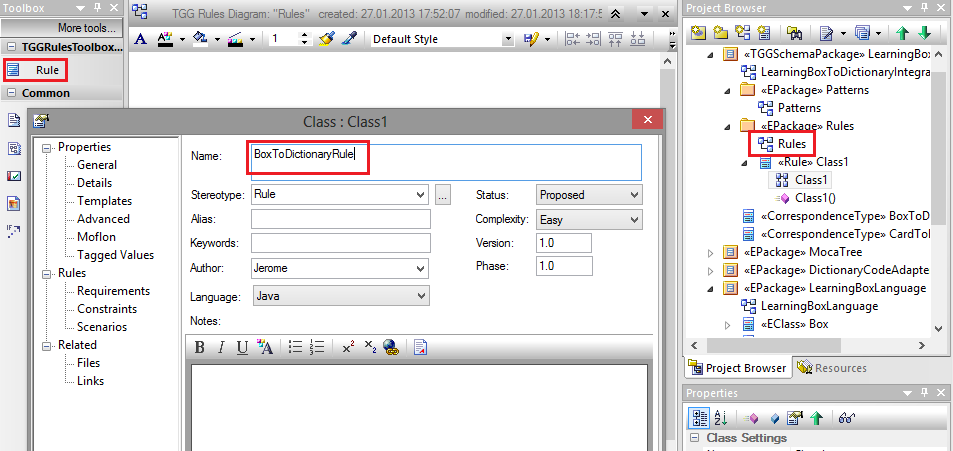
\includegraphics[width=\textwidth]{pics/tggBilder/tggRule/tgg8}
  \caption{Creating a TGG Rule}  
  \label{fig:create_tgg_rule}
\end{center}
\end{figure}

\end{enumerate}

As depicted in Fig.~\ref{fig:first_tgg_rule}, the newly created rule has a method and an underlying diagram (indicated by two small circles at the bottom right).
The generated method is the operation to be executed when the TGG rule is applied and the diagram is the place where we specify it.

\begin{figure}[htbp]
\begin{center}
  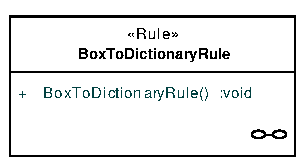
\includegraphics[width=0.35\textwidth]{pics/tggBilder/tggRule/tgg9}
  \caption{Our first TGG Rule}  
  \label{fig:first_tgg_rule}
\end{center}
\end{figure}

\begin{enumerate}
\item[$\blacktriangleright$] Double click our newly created \texttt{BoxToDictionaryRule} to open its diagram.
\item[$\blacktriangleright$] Drag \& drop a \texttt{Box} from project browser \texttt{as instance of element}, enter \texttt{box} as its name and choose \texttt{Create} as binding operator (Fig.~\ref{fig:create_tgg_object}).

\item[$\blacktriangleright$] In the same way, create an instance of \texttt{Dictionary} and name it \texttt{dictionary}.

\item[$\blacktriangleright$] Create also an instance of the correspondence type \texttt{BoxToDictionary} and name it \texttt{boxToDictionary}.
By quick link in EA, create links to source (\texttt{box}) and target (\texttt{dictionary}) objects, so that your diagram resembles Fig.~\ref{fig:first_rule_diagram}.

\begin{figure}[htbp]
\begin{center}
  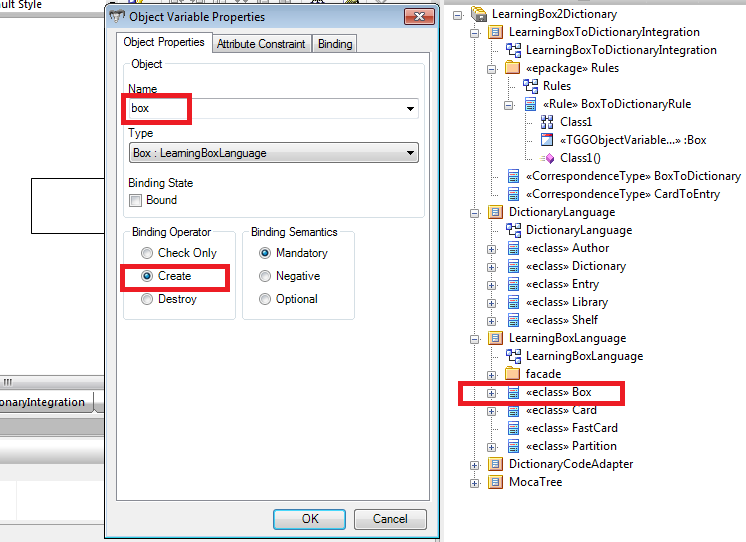
\includegraphics[width=\textwidth]{pics/tggBilder/tggRule/tgg10}
  \caption{Creating a TGG object variable}  
  \label{fig:create_tgg_object}
\end{center}
\end{figure}

\begin{figure}[htbp]
\begin{center}
  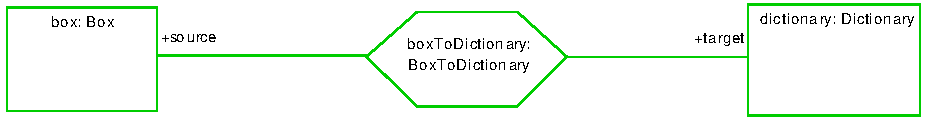
\includegraphics[width=\textwidth]{pics/tggBilder/tggRule/tgg11}
  \caption{TGG Rule Diagram after creating source, target and correspondence objects}  
  \label{fig:first_rule_diagram}
\end{center}
\end{figure}
\end{enumerate}

Now we have our first triple graph structure consisting of objects from each source, target and correspondence graphs.
We could interprete our diagram in Fig.~\ref{fig:first_rule_diagram} as follows:
``For each \texttt{Box} existing in source graph, a \texttt{Dictionary} in target graph is to be created, and vice versa. 
In both cases, a correspondence relating them to each other is also to be created in correspondence graph.''

A further plausible requirement for our TGG rule would be to keep the \texttt{name} attribute of a \texttt{Box} and the \texttt{title} attribute of a \texttt{Dictionary} consistently equal to each other.
\note{Attribute Constraints}
Our approach for this kind of requirements is \emph{attribute constraints} which provide a bidirectional and high-level solution for attribute manipulations.
In the next step we will define a constraint which applies to the objects \texttt{box} and \texttt{dictionary} and ensures the equality of \texttt{box.name} and \texttt{dictionary.title}.

\begin{enumerate}
\item[$\blacktriangleright$] In EA, drag \& drop a constraint from the Common Toolbox (Fig.~\ref{fig:common_toolbox}).

\begin{figure}[htbp]
\begin{center}
  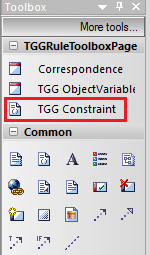
\includegraphics[width=0.25\textwidth]{pics/tggBilder/tggRule/tgg12}
  \caption{The Common Toolbox in EA}  
  \label{fig:common_toolbox}
\end{center}
\end{figure}

\item[$\blacktriangleright$] Double click the constraint element and enter \texttt{eq(box.name, dictionary.title)} as constraint as depicted in Fig.~\ref{fig:first_tgg_constraint}. 
Affirm with OK.

\begin{figure}[htbp]
\begin{center}
  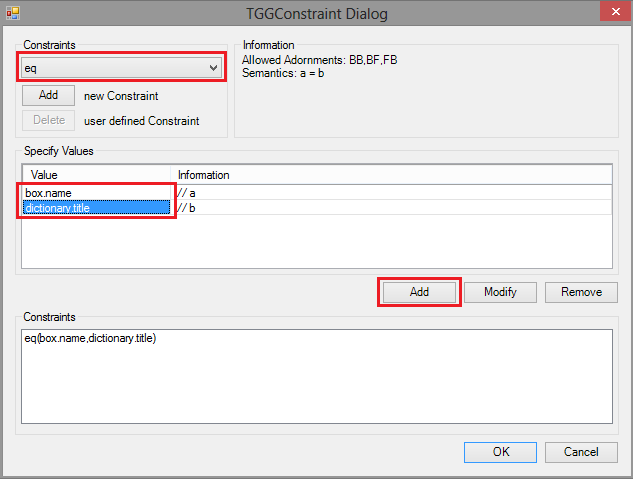
\includegraphics[width=0.5\textwidth]{pics/tggBilder/tggRule/tgg13}
  \caption{Creating a Constraint in EA}  
  \label{fig:first_tgg_constraint}
\end{center}
\end{figure}

\item[$\blacktriangleright$] Quick link a \texttt{Dependency} from the constraint to the both affected objects \texttt{box} and \texttt{dictionary}. 
Your TGG rule diagram should resemble Fig.~\ref{fig:tgg_rule_with_constraint}. 

\begin{figure}[htbp]
\begin{center}
  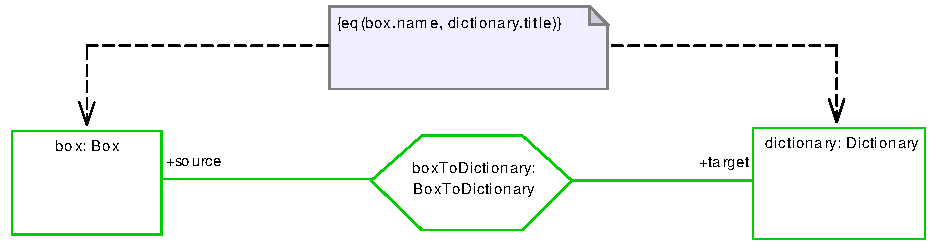
\includegraphics[width=\textwidth]{pics/tggBilder/tggRule/tgg14}
  \caption{A TGG Rule with a Constraint}  
  \label{fig:tgg_rule_with_constraint}
\end{center}
\end{figure}

\end{enumerate} 

The \texttt{eq} function, like any other constraint function we will discuss later, is bijective to ensure the reversibility and applies therefore to the both transformation directions, fulfilling the TGG philosophy of providing \emph{single} specification for unidirectional model transformation.

The last thing to do for our first TGG rule is to do some completions on the source side. 
On the target side, a \texttt{Dictionary} is a direct container for the \texttt{Entry} objects. But on the source side, solely a \texttt{Box} can't be sufficient to map the content of a \texttt{Dictionary}. 
In other words, a \texttt{Box} should contain \texttt{Partition}s to locate \texttt{Card}s. 
Only then is a \texttt{Box} the proper counterpart of a \texttt{Dictionary} in a model transformation. 
Assuming that we deal with \texttt{Box}es with three levels, we should add three \texttt{Partition} objects to the source graph. 

\begin{enumerate}
\item[$\blacktriangleright$] Create three \texttt{Partition} objects by drag \& drop from the project browser (as instance of element) with binding operator \texttt{Create} and pull also the appropriate links between the objects, so that your TGG rule diagram resembles Fig.~\ref{fig:boxtodictionaryrule_complete}.

\begin{figure}[htbp]
\begin{center}
  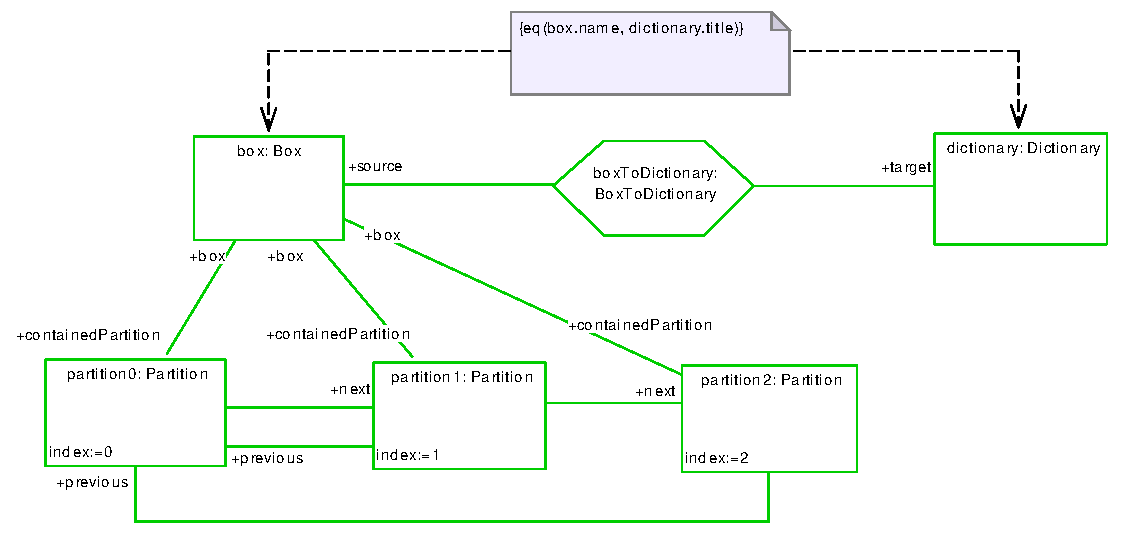
\includegraphics[width=\textwidth]{pics/tggBilder/tggRule/tgg15}
  \caption{Complete TGG rule diagram for \texttt{BoxToDictionaryRule}}  
  \label{fig:boxtodictionaryrule_complete}
\end{center}
\end{figure}

\end{enumerate}

Now, we will go deeper in the composite hierarchy of our metamodels and define our second and last TGG rule to specify the simultaneous evolution of \texttt{Card}, \texttt{Entry} and the correspondence \texttt{CardToEntry} between them.

\begin{enumerate}
\item[$\blacktriangleright$] Open \texttt{Rules} diagram again and create a new TGG Rule and name it \texttt{CardToEntryRule}.
\end{enumerate}

Your \texttt{Rules} diagram should resemble Fig.~\ref{fig:rules_diagram}.

\begin{figure}[htbp]
\begin{center}
  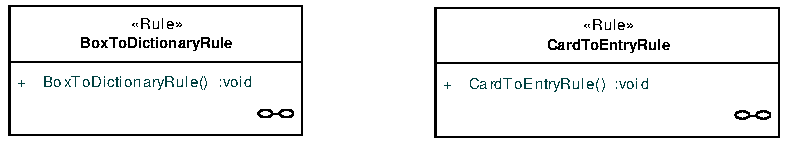
\includegraphics[width=\textwidth]{pics/tggBilder/tggRule/tgg16}
  \caption{The \texttt{Rules} diagram after creating two TGG Rules}  
  \label{fig:rules_diagram}
\end{center}
\end{figure}

Before specifying our second rule, we can describe our next goal as follows: ``Each \texttt{Card} in the \texttt{Partition}s of a \texttt{Box} should be transformed to an \texttt{Entry} of the corresponding \texttt{Dictionary}, and vice versa. 
In both cases, a correspondence \texttt{CardToEntry} should also be created''. 
That means, in our new rule we will first check the existence of bound objects from our first rule and then add our content objects (\texttt{Card} or \texttt{Entry}) to them.

\begin{enumerate}
\item[$\blacktriangleright$] Double click the newly created \texttt{CardToEntryRule} to open its diagram.
\item[$\blacktriangleright$] Drag \& drop an instance of \texttt{Box}, name it \texttt{box} and choose \texttt{Check only} as binding operator (Fig.~\ref{fig:bound_tgg_variable}).
\item[$\blacktriangleright$] In the same way, drag \& drop instances of \texttt{Partition}, \texttt{Dictionary} and \texttt{BoxToDictionary} and pull the appropriate links, so that your rule diagram resembles Fig.~\ref{fig:check_bound_variables}.

\begin{figure}[htbp]
\begin{center}
  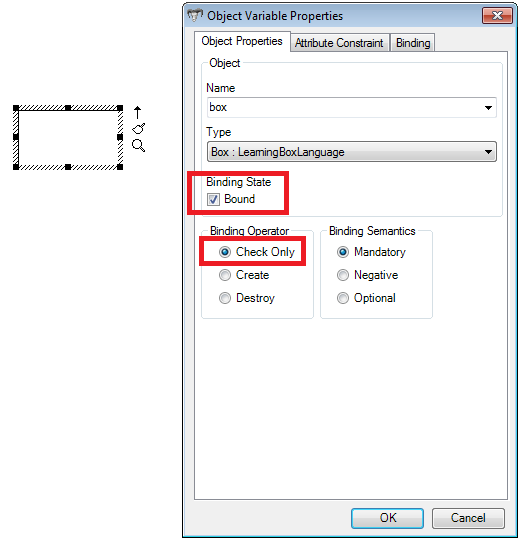
\includegraphics[width=0.6\textwidth]{pics/tggBilder/tggRule/tgg17}
  \caption{Creating a Check Only TGG Variable}  
  \label{fig:bound_tgg_variable}
\end{center}
\end{figure}

\begin{figure}[htbp]
\begin{center}
  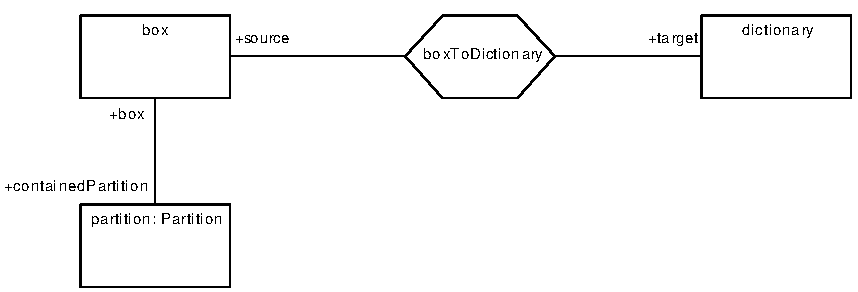
\includegraphics[width=\textwidth]{pics/tggBilder/tggRule/tgg18}
  \caption{checking the TGG Variables from other Rule }  
  \label{fig:check_bound_variables}
\end{center}
\end{figure}

\end{enumerate}

Now it's time to add our new objects to the graph triple in case of graph pattern matching. 

\begin{enumerate}
\item[$\blacktriangleright$] Complete your TGG Rule by creating \texttt{Card}, \texttt{Entry} and \texttt{CardToEntry} objects with binding operator \texttt{Create}, so that your TGG rule resembles Fig.~\ref{fig:cardtoentry_1}.

\begin{figure}[htbp]
\begin{center}
  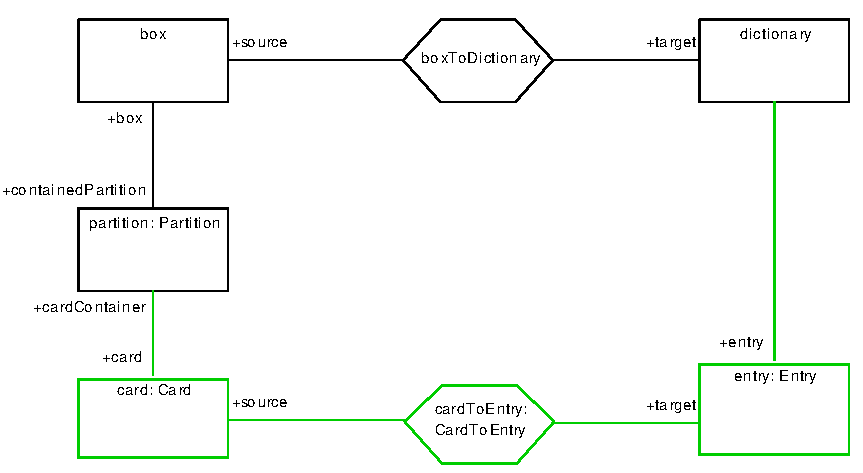
\includegraphics[width=\textwidth]{pics/tggBilder/tggRule/tgg19}
  \caption{TGG Rule \texttt{CardToEntryRule} without Attribute Manipulations}  
  \label{fig:cardtoentry_1}
\end{center}
\end{figure}

\end{enumerate}

The last thing to do for our second TGG rule is to define some attribute constraints for the transformarion between related \texttt{Card} and \texttt{Entry} objects.
Assuming that the \texttt{content} of an \texttt{Entry} in a \texttt{Dictionary} has the form \texttt{<word>: <meaning>}, while the \texttt{face} of a \texttt{Card} reads \texttt{Question: <word>} and the \texttt{back} reads \texttt{Answer: <meaning>}.
With our two predefined attribute constraint functions \texttt{addPrefix} and \texttt{concat}, we can do the appropriate prefix additions and string concatenations.

\begin{enumerate}
\item[$\blacktriangleright$] Darg \& drop a new constraint to your diagram and add the following three lines to it:

\begin{itemize}
\item[] \texttt{addPrefix(``Question: ``, word, card.face)} 
\item[] \texttt{addPrefix(``Answer: ``, meaning, card.back)} 
\item[] \texttt{concat(word, ``: ``, meaning, entry.content)} 
\end{itemize}

\end{enumerate}

The rule diagram after adding these constraints is depicted in Fig.~\ref{fig:cardtoentry_2}.

\begin{figure}[htbp]
\begin{center}
  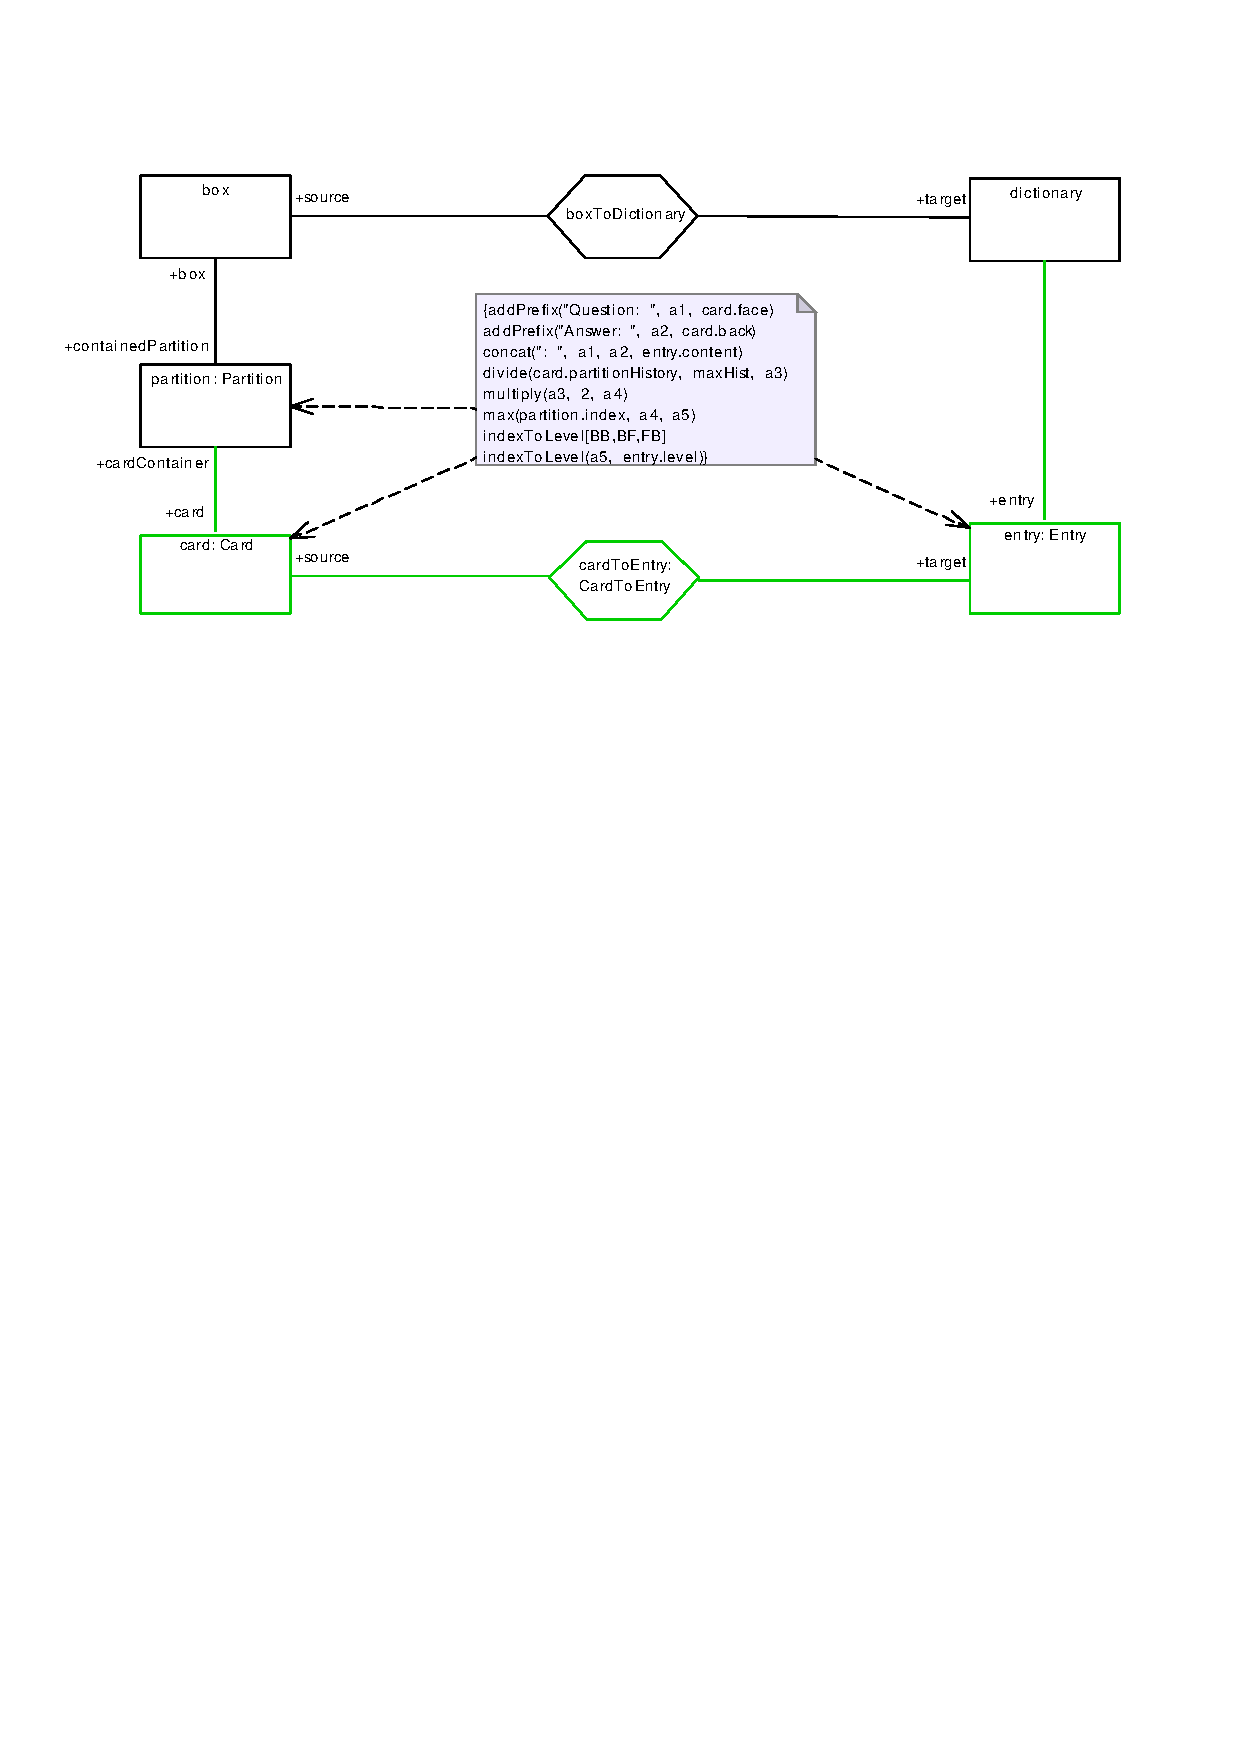
\includegraphics[width=\textwidth]{pics/tggBilder/tggRule/tgg20}
  \caption{String Manipulations for \texttt{card} and \texttt{entry}}  
  \label{fig:cardtoentry_2}
\end{center}
\end{figure}

The first attribute constraint of type \texttt{addPrefix} implies that \texttt{card.face} 
consists of a prefix \texttt{``Question :``} and a remaining part defined as variable \texttt{word}.
In the second attribute constraint, we use the same analogy for the \texttt{card.back} and define the variable \texttt{meaning}. 
And the third attribute constraint implies that the \texttt{entry.content} is the concatenation of these two variables with a colon in between.
These three attribute constraints are reversible (\emph{addPrefix vs. removePrefix} and \emph{concat vs. split}) and apply therefore to both transformation directions. 

The next question is how the dependence between \texttt{entry.\-level} and \texttt{par\-ti\-tion.\-index} looks like.
For example, a \texttt{Card} in a \texttt{Partition} with \texttt{index = 0} should be transformed to an \texttt{Entry} with level \texttt{beginner} and vice versa.
This time, we will define our own attribute constraint function which will be implemented later in hand-written Java code for the mapping between \texttt{partition.index} and \texttt{entry.level}. 

\begin{enumerate}
\item[$\blacktriangleright$]Darg \& drop a further constraint to your diagram and add the following two lines to it:

\begin{itemize}
\item[] \texttt{indexToLevel[BB,BF,FB]} 
\item[] \texttt{indexToLevel(partition.index, entry.level)} 
\end{itemize}

\end{enumerate}

In the end, be sure that your TGG rule resembles Fig.~\ref{fig:cardtoentry_complete} before you proceed to the next chapter.

\begin{figure}[htbp]
\begin{center}
  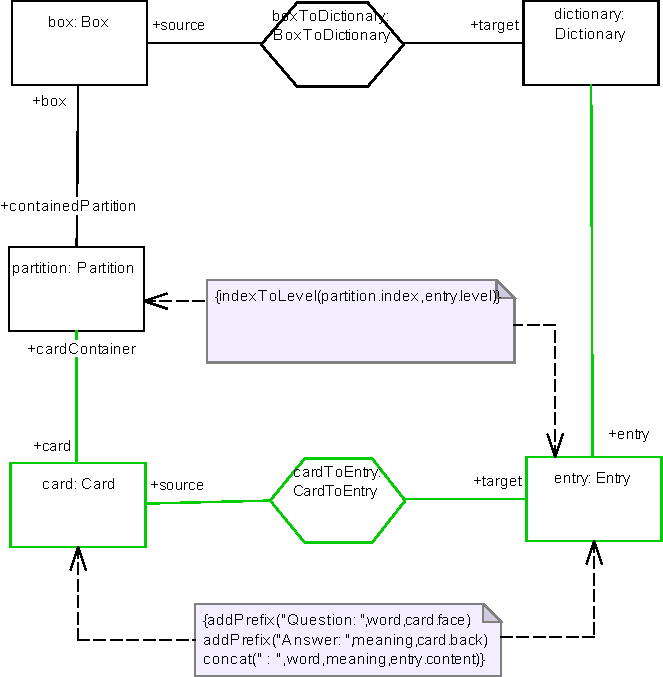
\includegraphics[width=\textwidth]{pics/tggBilder/tggRule/tgg21}
  \caption{Complete TGG Rule Diagram \texttt{CardToEntry}}  
  \label{fig:cardtoentry_complete}
\end{center}
\end{figure}

The new attribute constraint function \texttt{indexToLevel} will provide us a mapping between \texttt{partition.index} and \texttt{entry.level} by hand-written Java code. 
According to the declaration (first line) of our attribute constraint, we will distinguish between three different cases:

\begin{itemize}
\item[] \texttt{BB:} both \texttt{partition.index} and \texttt{entry.level} are \emph{bound}
\item[] \texttt{BF:} \texttt{partition.index} is \emph{bound} and \texttt{entry.level} is \emph{free}
\item[] \texttt{FB:} \texttt{partition.index} is \emph{free} and \texttt{entry.level} is \emph{bound} 
\end{itemize}